\documentclass[11pt,a4paper]{article}
\usepackage[margin=0.85in]{geometry}
\usepackage{amsmath}
\usepackage{graphicx}
\usepackage{booktabs}
\graphicspath{{output/figures/}}
\setlength{\parindent}{0pt}
\setlength{\parskip}{6pt}
\title{Polynomial Regression Assignment}
\author{Roll No.: IMT2024073}
\date{}

\begin{document}
\maketitle
\vspace{-1.5em}

\section{Approach}
In this assignment, I trained separate polynomial regression models for the two
problems. For \texttt{var1}, the aim was to predict the Net Power Score from six
plant operating parameters. For \texttt{var2}, the aim was to predict the Thermal
Anomaly Score from three spatial coordinates. I used the four datasets assigned
to my roll number, IMT2024073.

Each problem had 1,000 training samples and 1,000 test samples. The training
files contained the input features and the target $y$, while the test files
contained only the inputs. There were no missing values or exact duplicate
training rows. The features were already in the range $[-1,1]$, so I did not
apply further normalization.

\subsection{Polynomial model}
I included powers of each feature and interactions between features. For $p$
input variables, the model was
\[
  \hat y=\beta_0+
  \sum_{\substack{a_1,\ldots,a_p\geq 0\\1\leq a_1+\cdots+a_p\leq d}}
  \beta_{a_1,\ldots,a_p}\prod_{j=1}^{p}x_j^{a_j}.
\]
Here, $d$ is the maximum total degree. For example, $x_1^2x_2$ has degree 3,
and is included only when $d\geq 3$. This follows the degree definition in the
assignment. The number of nonconstant terms is $\binom{p+d}{d}-1$.

High degrees produce many terms compared with the number of training samples.
I therefore used regularization along with polynomial features. I compared
Ridge regression, which penalizes squared coefficients, and Lasso regression,
which penalizes absolute coefficients and can set some of them to zero. The
intercept was not penalized. Both methods still produce polynomial models.

\subsection{Choosing the model}
I split each training dataset into 800 samples for model selection and 200
samples for validation, using random seed 42. Within the 800 samples, I used
three-fold cross-validation with shuffling and seed 17. I selected the degree
and regularization strength using the lowest mean cross-validation MSE.
The 200 validation samples were not used to choose these settings.

For Ridge, I checked every degree from 1 to 10 for \texttt{var1}, and from 1
to 20 for \texttt{var2}. I also compared ordinary polynomial terms with a
Legendre polynomial basis. These bases represent the same polynomial space,
but regularization acts differently on their coefficients. The selected
models used ordinary polynomial terms.

\newpage
\section{Degree Selection and Regularization}
For Ridge, I used 13 values of $\alpha$, from $10^{-8}$ to $10^4$ in powers of
ten. For Lasso, I used $\alpha\in\{0.03,0.01,0.003,0.001\}$, with degrees
$\{3,5,7,10\}$ for \texttt{var1} and $\{6,10,14,20\}$ for \texttt{var2}.
Lasso settings that did not converge within the iteration limit in a
cross-validation fold were excluded. In total, I evaluated 812 configurations.

\begin{figure}[ht]
  \centering
  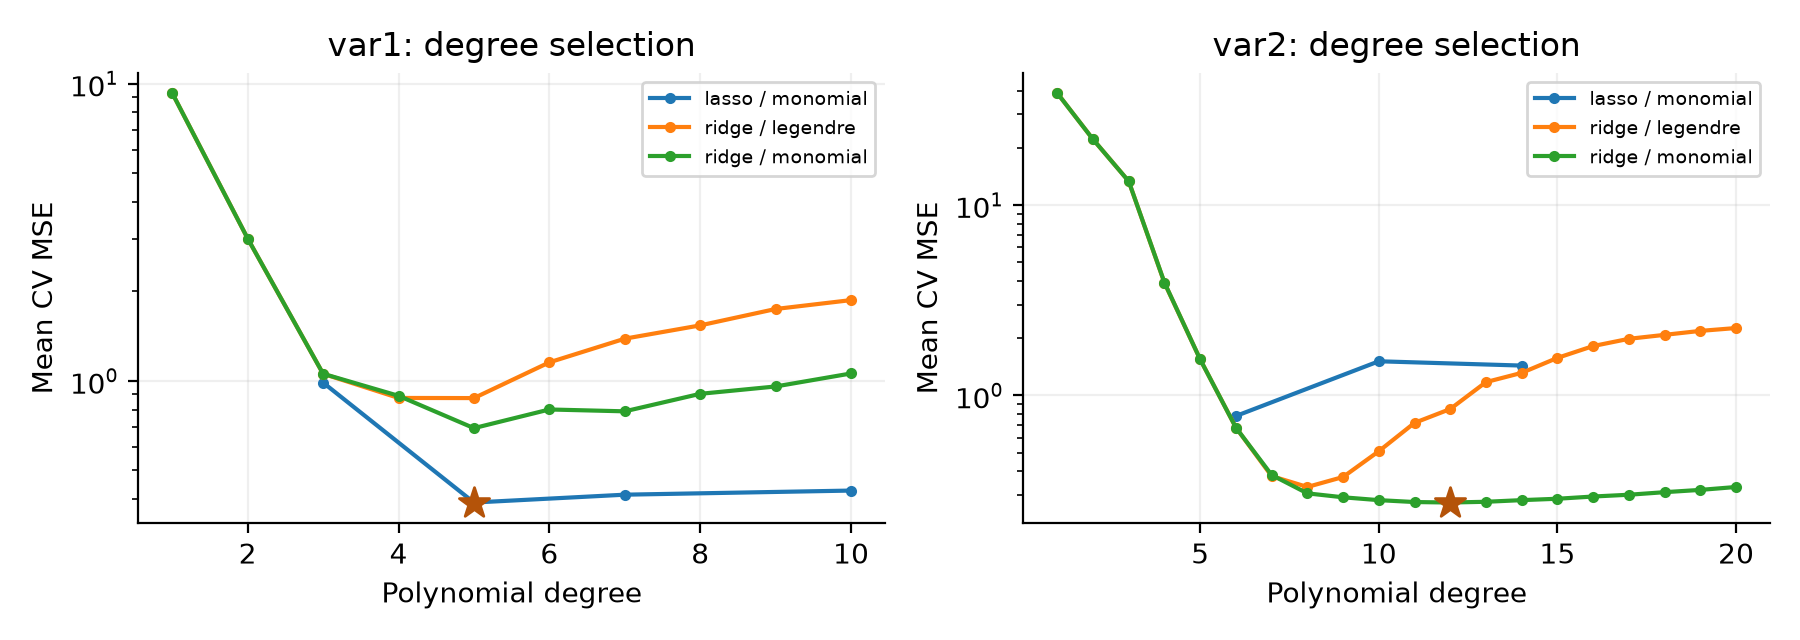
\includegraphics[width=\textwidth]{degree_selection.png}
  \caption{Cross-validation MSE against polynomial degree. Each curve uses the
  best tested $\alpha$ at that degree. The stars mark the selected models.}
\end{figure}

\subsection{Phase 1: Power Plant Steam Turbine Optimization (var1)}
I selected a degree-5 polynomial with Lasso regularization and
$\alpha=0.003$. Its mean cross-validation MSE was 0.38929. For comparison,
the best degree-5 Ridge model with ordinary polynomial terms had an MSE of
0.69282. The Lasso model gave a lower error while retaining fewer terms.

With six inputs, degree 5 gives 461 possible nonconstant terms. After fitting
the final model to all training samples, 121 coefficients were nonzero.
Increasing the degree did not improve the best cross-validation result.
For example, the best tested degree-7 Lasso model had an MSE of about 0.41367.
I therefore chose degree 5 instead of using the maximum allowed degree of 10.

\subsection{Phase 2: Subterranean Thermal Reservoir Mapping (var2)}
I selected a degree-12 polynomial with Ridge regularization and
$\alpha=0.1$. Its mean cross-validation MSE was 0.27312. Lower degrees did not
fit this dataset as well: the best ordinary-basis Ridge MSE was 0.67683 at
degree 6 and 0.28111 at degree 10.

The error reached its lowest value at degree 12 and increased gradually after
that. At degree 20, the best ordinary-basis Ridge MSE was 0.32966. I chose
degree 12 because it gave the lowest cross-validation error, rather than
assuming that the highest permitted degree would be the most accurate.
This model has 454 nonconstant terms. Lasso did not improve on the selected
Ridge model for this problem.

\newpage
\section{Results}
After selecting the models, I fitted them on the 800 model-selection samples
and evaluated them on the remaining 200 validation samples. I used the two
metrics specified in the assignment:
\[
\mathrm{MSE}=\frac{1}{n}\sum_{i=1}^{n}(y_i-\hat y_i)^2,
\qquad
R^2=1-\frac{\sum_{i=1}^{n}(y_i-\hat y_i)^2}
                  {\sum_{i=1}^{n}(y_i-\bar y)^2}.
\]

\begin{table}[ht]
\centering
\begin{tabular}{lccccc}
\toprule
Problem & Degree & Method & $\alpha$ & Validation MSE & Validation $R^2$ \\
\midrule
\texttt{var1} & 5 & Lasso & 0.003 & 0.37664 & 0.96687 \\
\texttt{var2} & 12 & Ridge & 0.1 & 0.24579 & 0.99507 \\
\bottomrule
\end{tabular}
\caption{Results on the 200 reserved validation samples for each problem.}
\end{table}

As a simple baseline, I predicted the mean target value from the 800
model-selection samples. This gave validation MSE values of 11.37616 for
\texttt{var1} and 50.62658 for \texttt{var2}. Both polynomial models reduced
the error substantially compared with this baseline.

\begin{figure}[ht]
\centering
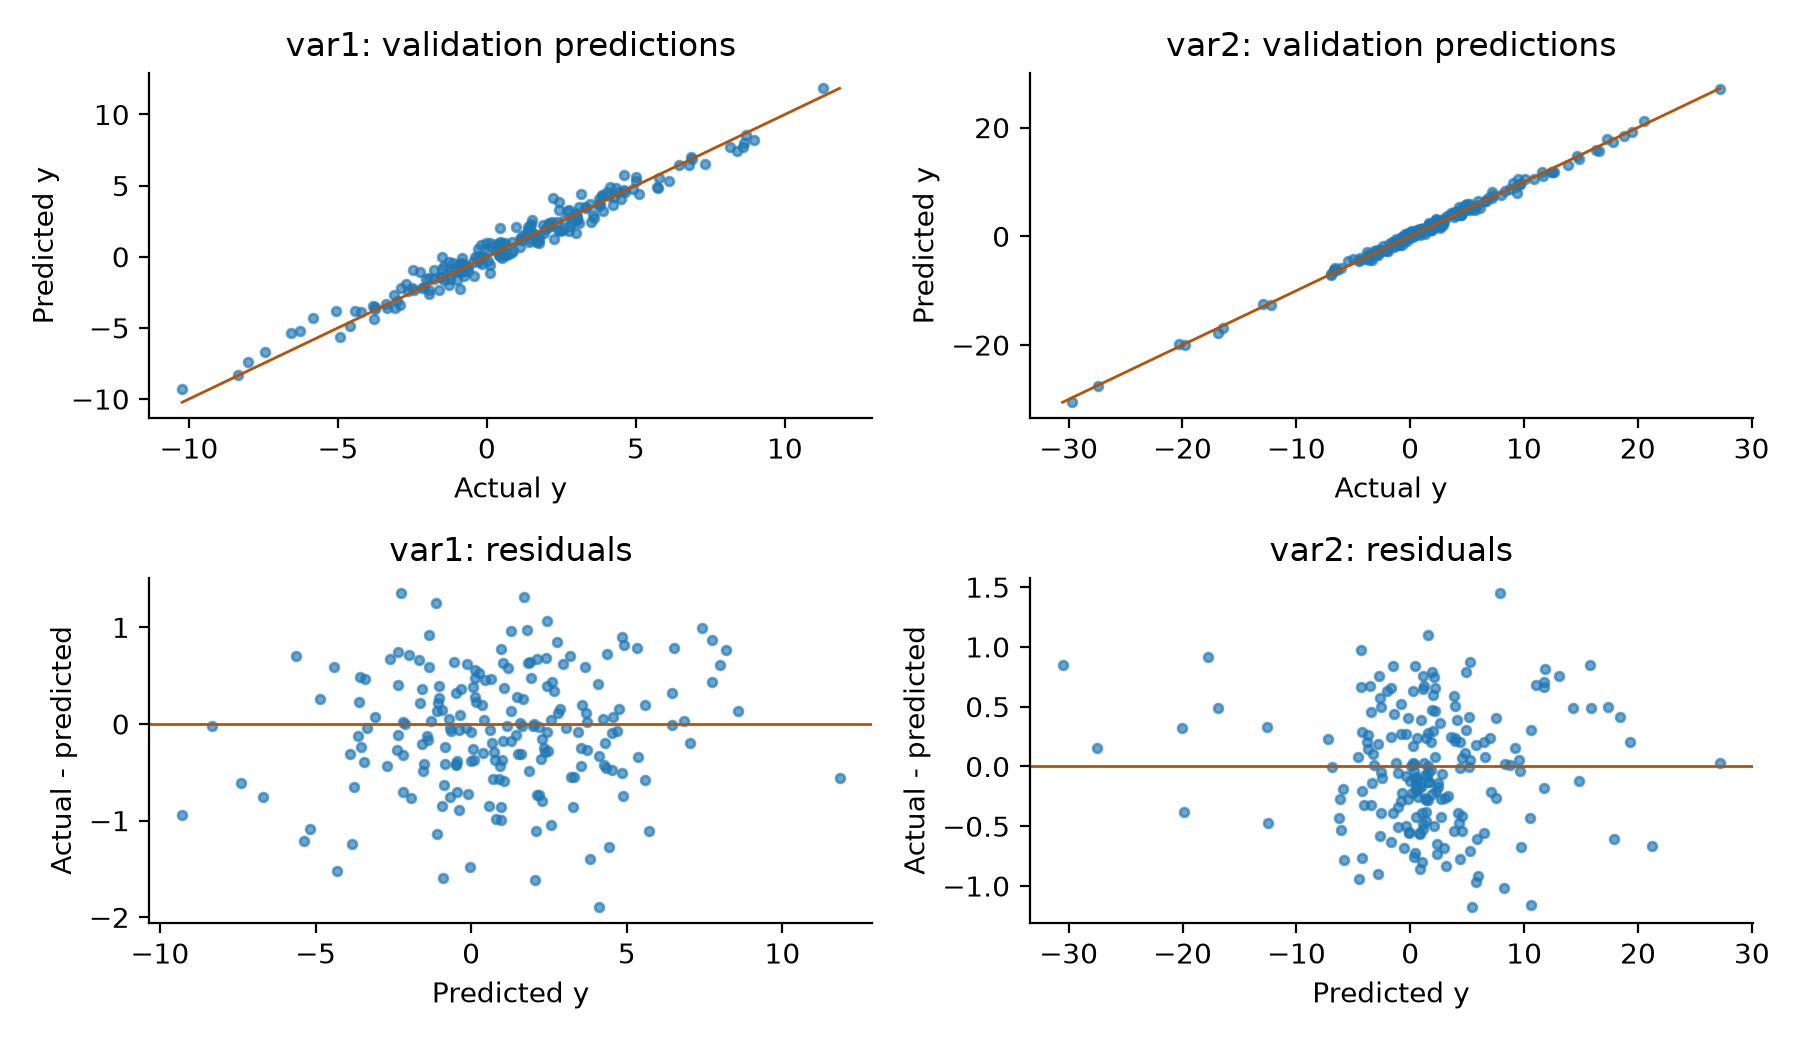
\includegraphics[width=0.94\textwidth]{holdout_diagnostics.png}
\caption{Predicted and actual validation targets, and the corresponding
residuals. Predictions close to the diagonal have smaller errors.}
\end{figure}

\section{Final Predictions}
I refitted each selected model on all 1,000 training samples and predicted
$y$ for its corresponding test dataset. The submitted files are
\texttt{IMT2024073\_pred\_var1.csv} and
\texttt{IMT2024073\_pred\_var2.csv}. Each contains 1,000 rows and a single
\texttt{y} column, matching \texttt{sample\_submission.csv}. I kept the
original test-row order.

The reported scores are validation scores, since the test targets are hidden.
In particular, the \texttt{var1} test inputs have a greater spread than the
training inputs, so the test error may differ from the validation error.
The repository contains the training and inference code, along with the
cross-validation results and the LaTeX source of this report.

\end{document}
